\documentclass{standalone}
\usepackage{tikz}
\usetikzlibrary{patterns, positioning}

\begin{document}
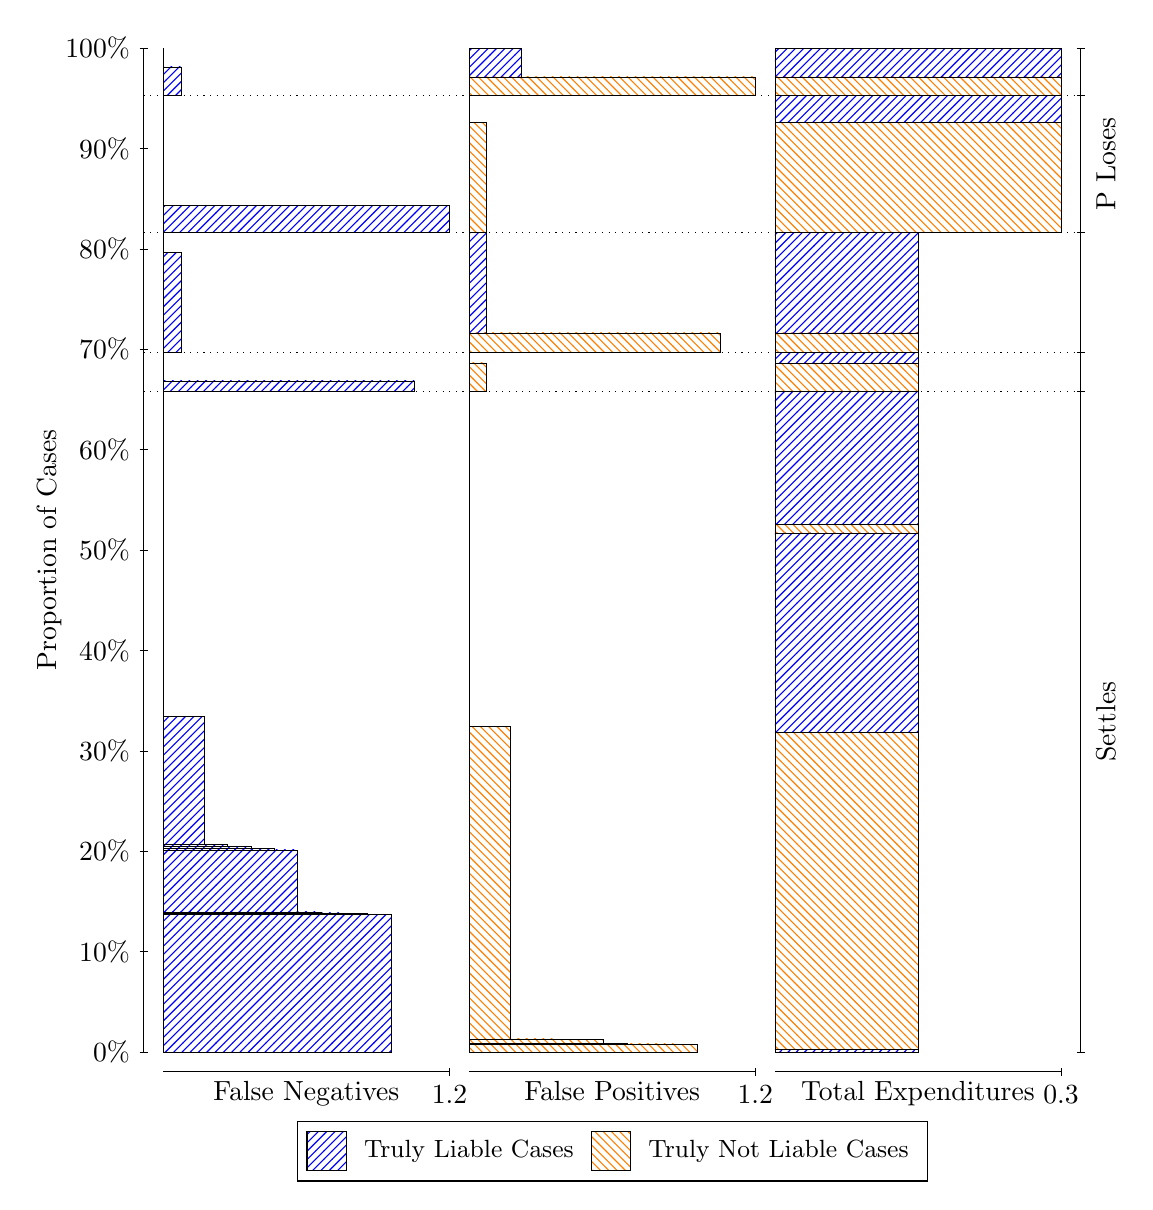
\begin{tikzpicture}
\draw[black, very thin] (1.5,1.75) -- (1.5,14.5);
\node[rotate=90, anchor=center] at (0.3, 8.125) {Proportion of Cases};
\draw[black, very thin] (1.45,1.75) -- (1.55,1.75);
\node[anchor=east] at (1.45, 1.75) {0\%};
\draw[black, very thin] (1.45,3.025) -- (1.55,3.025);
\node[anchor=east] at (1.45, 3.025) {10\%};
\draw[black, very thin] (1.45,4.3) -- (1.55,4.3);
\node[anchor=east] at (1.45, 4.3) {20\%};
\draw[black, very thin] (1.45,5.575) -- (1.55,5.575);
\node[anchor=east] at (1.45, 5.575) {30\%};
\draw[black, very thin] (1.45,6.85) -- (1.55,6.85);
\node[anchor=east] at (1.45, 6.85) {40\%};
\draw[black, very thin] (1.45,8.125) -- (1.55,8.125);
\node[anchor=east] at (1.45, 8.125) {50\%};
\draw[black, very thin] (1.45,9.4) -- (1.55,9.4);
\node[anchor=east] at (1.45, 9.4) {60\%};
\draw[black, very thin] (1.45,10.675) -- (1.55,10.675);
\node[anchor=east] at (1.45, 10.675) {70\%};
\draw[black, very thin] (1.45,11.95) -- (1.55,11.95);
\node[anchor=east] at (1.45, 11.95) {80\%};
\draw[black, very thin] (1.45,13.225) -- (1.55,13.225);
\node[anchor=east] at (1.45, 13.225) {90\%};
\draw[black, very thin] (1.45,14.5) -- (1.55,14.5);
\node[anchor=east] at (1.45, 14.5) {100\%};

\draw[black, very thin] (13.4,1.75) -- (13.4,14.5);
\draw[black, very thin] (13.35,1.75) -- (13.45,1.75);
\node[anchor=west] at (13.35, 1.75) {};
\draw[black, very thin] (13.35,10.14) -- (13.45,10.14);
\node[anchor=west] at (13.35, 10.14) {};
\draw[black, very thin] (13.35,10.632) -- (13.45,10.632);
\node[anchor=west] at (13.35, 10.632) {};
\draw[black, very thin] (13.35,12.155) -- (13.45,12.155);
\node[anchor=west] at (13.35, 12.155) {};
\draw[black, very thin] (13.35,13.894) -- (13.45,13.894);
\node[anchor=west] at (13.35, 13.894) {};
\draw[black, very thin] (13.35,14.5) -- (13.45,14.5);
\node[anchor=west] at (13.35, 14.5) {};

\draw[black, very thin, pattern color=blue, pattern=north east lines] (1.75,1.75) rectangle (4.6418,3.4949);
\draw[black, very thin, pattern color=blue, pattern=north east lines] (1.75,3.4949) rectangle (4.3452,3.5058);
\draw[black, very thin, pattern color=blue, pattern=north east lines] (1.75,3.5058) rectangle (4.0486,3.5176);
\draw[black, very thin, pattern color=blue, pattern=north east lines] (1.75,3.5176) rectangle (3.752,3.5301);
\draw[black, very thin, pattern color=blue, pattern=north east lines] (1.75,3.5301) rectangle (3.4554,4.3153);
\draw[black, very thin, pattern color=blue, pattern=north east lines] (1.75,4.3153) rectangle (3.1588,4.3378);
\draw[black, very thin, pattern color=blue, pattern=north east lines] (1.75,4.3378) rectangle (2.8622,4.3607);
\draw[black, very thin, pattern color=blue, pattern=north east lines] (1.75,4.3607) rectangle (2.5656,4.3839);
\draw[black, very thin, pattern color=blue, pattern=north east lines] (1.75,4.3839) rectangle (2.269,6.009);
\draw[black, very thin, pattern color=orange, pattern=north west lines] (1.75,6.009) rectangle (1.75,10.14);
\draw[black, very thin, pattern color=blue, pattern=north east lines] (1.75,10.14) rectangle (4.9384,10.272);
\draw[black, very thin, pattern color=orange, pattern=north west lines] (1.75,10.272) rectangle (1.75,10.632);
\draw[black, very thin, pattern color=blue, pattern=north east lines] (1.75,10.632) rectangle (1.9724,11.906);
\draw[black, very thin, pattern color=orange, pattern=north west lines] (1.75,11.906) rectangle (1.75,12.155);
\draw[black, very thin, pattern color=blue, pattern=north east lines] (1.75,12.155) rectangle (5.3833,12.498);
\draw[black, very thin, pattern color=orange, pattern=north west lines] (1.75,12.498) rectangle (1.75,13.894);
\draw[black, very thin, pattern color=blue, pattern=north east lines] (1.75,13.894) rectangle (1.9724,14.261);
\draw[black, very thin, pattern color=orange, pattern=north west lines] (1.75,14.261) rectangle (1.75,14.5);
\draw[black, very thin, pattern color=orange, pattern=north west lines] (5.6333,1.75) rectangle (8.5252,1.8504);
\draw[black, very thin, pattern color=orange, pattern=north west lines] (5.6333,1.8504) rectangle (8.2286,1.8521);
\draw[black, very thin, pattern color=orange, pattern=north west lines] (5.6333,1.8521) rectangle (7.932,1.8538);
\draw[black, very thin, pattern color=orange, pattern=north west lines] (5.6333,1.8538) rectangle (7.6354,1.8555);
\draw[black, very thin, pattern color=orange, pattern=north west lines] (5.6333,1.8555) rectangle (7.3388,1.9137);
\draw[black, very thin, pattern color=orange, pattern=north west lines] (5.6333,1.9137) rectangle (7.0422,1.9137);
\draw[black, very thin, pattern color=orange, pattern=north west lines] (5.6333,1.9137) rectangle (7.0422,1.9146);
\draw[black, very thin, pattern color=orange, pattern=north west lines] (5.6333,1.9146) rectangle (6.7456,1.9154);
\draw[black, very thin, pattern color=orange, pattern=north west lines] (5.6333,1.9154) rectangle (6.449,1.9161);
\draw[black, very thin, pattern color=orange, pattern=north west lines] (5.6333,1.9161) rectangle (6.1524,5.8812);
\draw[black, very thin, pattern color=blue, pattern=north east lines] (5.6333,5.8812) rectangle (5.6333,10.14);
\draw[black, very thin, pattern color=orange, pattern=north west lines] (5.6333,10.14) rectangle (5.8558,10.5);
\draw[black, very thin, pattern color=blue, pattern=north east lines] (5.6333,10.5) rectangle (5.6333,10.632);
\draw[black, very thin, pattern color=orange, pattern=north west lines] (5.6333,10.632) rectangle (8.8218,10.881);
\draw[black, very thin, pattern color=blue, pattern=north east lines] (5.6333,10.881) rectangle (5.8558,12.155);
\draw[black, very thin, pattern color=orange, pattern=north west lines] (5.6333,12.155) rectangle (5.8558,13.551);
\draw[black, very thin, pattern color=blue, pattern=north east lines] (5.6333,13.551) rectangle (5.6333,13.894);
\draw[black, very thin, pattern color=orange, pattern=north west lines] (5.6333,13.894) rectangle (9.2667,14.133);
\draw[black, very thin, pattern color=blue, pattern=north east lines] (5.6333,14.133) rectangle (6.3007,14.5);
\draw[black, very thin, pattern color=orange, pattern=north west lines] (9.5167,1.75) rectangle (11.333,1.7524);
\draw[black, very thin, pattern color=blue, pattern=north east lines] (9.5167,1.7524) rectangle (11.333,1.7877);
\draw[black, very thin, pattern color=orange, pattern=north west lines] (9.5167,1.7877) rectangle (11.333,5.811);
\draw[black, very thin, pattern color=blue, pattern=north east lines] (9.5167,5.811) rectangle (11.333,8.341);
\draw[black, very thin, pattern color=orange, pattern=north west lines] (9.5167,8.341) rectangle (11.333,8.4465);
\draw[black, very thin, pattern color=blue, pattern=north east lines] (9.5167,8.4465) rectangle (11.333,10.14);
\draw[black, very thin, pattern color=orange, pattern=north west lines] (9.5167,10.14) rectangle (11.333,10.5);
\draw[black, very thin, pattern color=blue, pattern=north east lines] (9.5167,10.5) rectangle (11.333,10.632);
\draw[black, very thin, pattern color=orange, pattern=north west lines] (9.5167,10.632) rectangle (11.333,10.881);
\draw[black, very thin, pattern color=blue, pattern=north east lines] (9.5167,10.881) rectangle (11.333,12.155);
\draw[black, very thin, pattern color=orange, pattern=north west lines] (9.5167,12.155) rectangle (13.15,13.551);
\draw[black, very thin, pattern color=blue, pattern=north east lines] (9.5167,13.551) rectangle (13.15,13.894);
\draw[black, very thin, pattern color=orange, pattern=north west lines] (9.5167,13.894) rectangle (13.15,14.133);
\draw[black, very thin, pattern color=blue, pattern=north east lines] (9.5167,14.133) rectangle (13.15,14.5);
\draw[black, dotted] (1.5,10.14) -- (13.4,10.14);
\draw[black, dotted] (1.5,10.632) -- (13.4,10.632);
\draw[black, dotted] (1.5,12.155) -- (13.4,12.155);
\draw[black, dotted] (1.5,13.894) -- (13.4,13.894);
\draw[black, very thin] (1.75,1.5) -- (5.3833,1.5);
\node[anchor=north] at (3.5667, 1.5) {False Negatives};
\draw[black, very thin] (5.3833,1.45) -- (5.3833,1.55);
\node[anchor=north] at (5.3833, 1.45) {1.2};

\draw[black, very thin] (5.6333,1.5) -- (9.2667,1.5);
\node[anchor=north] at (7.45, 1.5) {False Positives};
\draw[black, very thin] (9.2667,1.45) -- (9.2667,1.55);
\node[anchor=north] at (9.2667, 1.45) {1.2};

\draw[black, very thin] (9.5167,1.5) -- (13.15,1.5);
\node[anchor=north] at (11.333, 1.5) {Total Expenditures};
\draw[black, very thin] (13.15,1.45) -- (13.15,1.55);
\node[anchor=north] at (13.15, 1.45) {0.3};

\node[black, centered, rotate=90] at (13.72, 5.9451) {Settles};


\node[black, centered, rotate=90] at (13.72, 13.025) {P Loses};


\draw (7.449999999999999,1.5) node[draw=none] (baseCoordinate) {};
\begin{scope}[align=center]
        \matrix[scale=0.5, draw=black, below=0.5cm of baseCoordinate, nodes={draw}, column sep=0.1cm]{
            \node[rectangle, draw, minimum width=0.5cm, minimum height=0.5cm, pattern=north east lines, pattern color=blue] {}; &
            \node[draw=none, font=\small] (B) {Truly Liable Cases}; &
            \node[rectangle, draw, minimum width=0.5cm, minimum height=0.5cm, pattern=north west lines, pattern color=orange] {}; &
            \node[draw=none, font=\small] (B) {Truly Not Liable Cases}; \\
            };
\end{scope}

\end{tikzpicture}
\end{document}